 \begin{tikzpicture}[overlay, remember picture]
        \node[circle, fill=black, inner sep=2pt, label=above:$A$] at (current page.north east) [xshift=-2cm, yshift=-2cm] (A) {};
        \node[circle, fill=black, inner sep=2pt, label=above:$B$] at (current page.north east) [xshift=-1cm, yshift=-2cm] (B) {};
        \draw (A) -- (B);
\end{tikzpicture}



\begin{itemize}
    \iitem  Pure states $\ket{\psi_{AB}}$: 
        \begin{itemize}
            \iitem{\textit{Product state} if $\ket{\psi_{AB}} = \ket{\psi_A} \otimes \ket{\psi_B}$}
            \iitem{$A$ is entangled with $B$ otherwise}
        \end{itemize}
    \vspace{3mm}
    \iitem Mixed states $\hat{\rho}_{AB}$
    \begin{itemize}
        \iitem{\textit{Separable state} if $\hat{\rho}_{AB} = \sum_k p_k \hat{\rho}_A^k \otimes \hat{\rho}_B^k$}
        \iitem{$A$ is entangled with $B$ otherwise}
    \end{itemize}
\end{itemize}

\vfill

\begin{figure}[h]
    \centering
    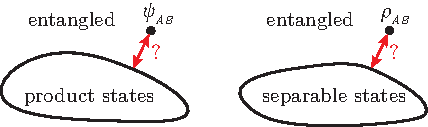
\includegraphics{imgs/Asset 2.pdf}
    %\caption{}
    %\label{fig:}
\end{figure}


% \begin{minipage}{0.45\textwidth}
%     \begin{block}{Entangled}
        
%     \end{block}
% \end{minipage}
% \hfill
% \begin{minipage}{0.45\textwidth}
%     \begin{block}{Non-entangled states}
%         For pure states: 
%     \end{block}
% \end{minipage}
%     